\documentclass[a4paper,12pt]{article}

\usepackage[english]{babel}
\usepackage[utf8]{inputenc}
\usepackage[T1]{fontenc}
\usepackage{graphicx}
\usepackage{rotating}
\usepackage{subfig}
\usepackage[pdftex]{hyperref}

\graphicspath{{images/}}

\hypersetup{
    bookmarks=false,           % show bookmarks bar?
    unicode=false,             % non-Latin characters in Acrobat's bookmarks
    pdftoolbar=true,           % show Acrobat's toolbar?
    pdfmenubar=true,           % show Acrobat's menu?
    pdffitwindow=false,        % page fit to window when opened
    pdftitle={Svg2tex Documentation}, % title
    pdfauthor={Lorenzo Tozzi}, % author
    %pdfsubject={},            % subject of the document
    pdfnewwindow=false,        % links in new window
    %pdfkeywords={},           % list of keywords
    colorlinks=true,           % false: boxed links; true: colored links
    linkcolor=black,           % color of internal links
    citecolor=black,           % color of links to bibliography
    filecolor=black,           % color of file links
    urlcolor=black             % color of external links
}

\begin{document}

\title{Svg2tex Documentation}

\author{Lorenzo Tozzi}
\date{\today}
\maketitle

\tableofcontents

\section{Licence}

Svg2tex is released under the GNU/GPL version 2 license. Svg2tex is free software.

\section{Intorduction}

When I was writing my thesis with \LaTeX , I wanted to include pictures in a vector format with the following features:
\begin{enumerate}
  \item easily edit pictures without loosing too much time;
  \item use \LaTeX\ commands inside pictures, even custom ones defined in the main document;
  \item have a consistent font and font size across the document, even inside pictures;
  \item change font and font size without having to re-edit every picture; ideally just editing \LaTeX\ document's header.
\end{enumerate}
I didn't find a suitable solution for all those issues, and that's why I've created svg2tex.

Svg2tex is a python script that extracts all text from a *.svg file to a \LaTeX\ picture environment. This way the picture's text is processed directly by \LaTeX\ and can be included into the document. Figure \ref{fig:comparison} compares the final result with and without svg2tex.
\begin{figure}[tb]
  \centering
  \subfloat[Not processed by svg2tex]{\label{fig:no_svg2tex}\includegraphics{comparison_bad}}
  \subfloat[Processed by svg2tex]{\label{fig:with_svg2tex}\setlength{\unitlength}{0.282222229121mm}
\begin{picture}(231.85715, 146.14285)(0, -146.14285)
  \put(0,-146.14285){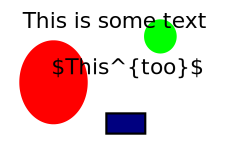
\includegraphics[height=41.2447608971mm, width=65.4352417106mm]{comparison}}
  \put(114.579643,-27.78134){\turnbox{-0.0}{\makebox(0,0)[bc]{This is some text}}}
  \put(128.013013,-74.43128){\turnbox{-0.0}{\makebox(0,0)[bc]{$This^{too}$}}}
\end{picture}}
  \caption{Pictures comparison}
  \label{fig:comparison}
\end{figure}

\section{Usage}

Svg2tex can be used as an inkscape extension or as a standalone script. The final result is the same.

\subsection{Inkscape extension}

Installing svg2tex is very easy. Under Linux you only need to copy \texttt{svg2tex.py} and \texttt{tex\_output.inx} under ``\texttt{/home/<your username>/.inkscape/extensions}''. Under Windows just copy the same files under ``\texttt{C:\textbackslash<inkscape installation directory>\textbackslash share\textbackslash extensions\textbackslash}''. At this point it's necessary to restart inkscape. Under the save menu there should be a new option: ``\emph{LaTeX (text only) picture environment (*.tex)}''.

As an example we will create a simple picture as shown in picture \ref{fig:inkscape_tutorial_pic}.
\begin{figure}[tb]
  \centering
  
\includegraphics{tutorial_1}
  \caption{The example document}
  \label{fig:inkscape_tutorial_pic}
\end{figure}
The first two lines have different sizes, while the third one has a \LaTeX\ command in it. At this point click on ``\emph{Save}'' and choose ``\emph{LaTeX (text only) picture environment (*.tex)}''. Set the file name as \texttt{example.tex} and click ``\emph{Save}''. We will be prompted with a pop-up window as in picture \ref{fig:inkscape_screenshot}.
\begin{figure}[tb]
  \centering
  \includegraphics[width=0.7\textwidth]{tutorial_2}
  \caption{Inkscape pop-up}
  \label{fig:inkscape_screenshot}
\end{figure}
For now leave it empty.

The newly created file can now be imported into a \LaTeX\ document with the following code:
\begin{verbatim}
\begin{figure}
  \centering
  \input{example.tex}
  \caption{This is an exaple file}
  \label{fig:example_label}
\end{figure}
\end{verbatim}

The main document must include \texttt{graphicx} and \texttt{rotating} packages in order to safely include pictures generated with svg2tex. The final result can be seen in picture \ref{fig:inkscape_tutorial_result_1}. As you can see, the red shapes are missing. This happens because svg2tex only converts *.svg document's text. The rest of the image must be loaded as a ``background''.
\begin{figure}[tb]
  \centering
  \input{images/tutorial_1_tex}
  \caption{Svg2tex output}
  \label{fig:inkscape_tutorial_result_1}
\end{figure}

Now go back to inkscape and overwrite \texttt{example.tex}. This time, when we are prompted with the pop-up window that asks for a background image (picture \ref{fig:inkscape_screenshot}) type in ``\texttt{example\_bg}''. At this stage \texttt{example.tex} is waiting for a background image called ``\texttt{example\_bg}'' (file extension is added by \LaTeX).

We must decide which file format to use for that background. \LaTeX\ can import a wide range of vector or raster images such as *.eps, *.png and *.jpeg. It depends if we are using ``\texttt{latex}'' or ``\texttt{pdflatex}'' to compile our document. More informations here: \url{http://en.wikibooks.org/wiki/LaTeX/Importing_Graphics}. Choosing the appropriate format is outside the scope of this document. We are importing the picture as a vector image and we are using the *.pdf format.

Now we must delete all text from the picture (it's already in our document, at this step we only need the red shapes) and click on ``\emph{Save}''. We have told to \texttt{example.tex} that the background image is called ``\texttt{example\_bg}'' so the filename must be \texttt{example\_bg.pdf} and must be placed in the same directory of \texttt{example.tex}. As the file format we choose ``\emph{PDF via Cairo (*.pdf)}''. The final result is shown in picture \ref{fig:inkscape_final_example}.
\begin{figure}[tb]
  \centering
  \setlength{\unitlength}{0.282222229121mm}
\begin{picture}(225.64949, 279.45886)(0, -279.45886)
  \put(0,-279.45886){\includegraphics[height=78.8695024168mm, width=63.6833020678mm]{tutorial_bg}}
  \put(10.76657,-116.28915){\turnbox{-0.0}{\makebox(0,0)[bl]{This is a big text}}}
  \put(19.0146,-231.37854){\turnbox{-0.0}{\makebox(0,0)[bl]{{\huge No, this is a big text}}}}
  \put(24.15159,-38.9779){\turnbox{-0.0}{\makebox(0,0)[bl]{Hello!}}}
\end{picture}
  \caption{Svg2tex output with the proper background}
  \label{fig:inkscape_final_example}
\end{figure}

As expected, the font and the font size is consistent with the rest of the document, so inkscape's preferences are ignored and the first two lines have the same height. At the same time the \LaTeX\ command \texttt{\textbackslash huge} is correctly processed and the third line is bigger than the others.

\subsection{Command-line}

Svg2tex can also be called from command-line. Here it is the syntax:
\begin{verbatim}
python svg2tex.py <options> <svg-input-file> <tex-output-file>
\end{verbatim}
The \texttt{<tex-output-file>} is optional and, if it's not given, the \LaTeX\ output is printed in standard output. The \texttt{<options>} can be any of the following:
\begin{itemize}
  \item \texttt{-i <filename>} (or \texttt{-{}-include <filename>}) -- set the background image of the picture environment to \texttt{<filename>}. It's the same as entering \texttt{<filename>} in inkscape as seen in picture \ref{fig:inkscape_screenshot};
  \item \texttt{-t <filename>} (or \texttt{-{}-textless <filename>}) -- make a copy of the original *.svg file without text and save it as \texttt{<filename>}.
\end{itemize}
Even from command-line, svg2tex can be paired with inkscape. The next simple shell script, for example, converts all *.svg files in the directory into ready-to-use \LaTeX\ + *.pdf pictures:
{\small
\begin{verbatim}
#!/bin/sh

for file in *.svg
do
  echo "Processing ${file}..."
  fn=${file%.svg}
  python svg2tex.py -i "${fn}" -t "${fn}.tl.svg" "${file}" "${fn}.tex"
  inkscape --export-pdf="${fn}.pdf" "${fn}.tl.svg"

  rm "${fn}.tl.svg"
done
\end{verbatim}
}

\section{Conclusion}

While I was working on svg2tex I focused around the command-line approach because it's a lot faster. It's possible to edit any of the *.svg files and run a simple shell script (like the one provided in this document) to update both, the *.tex and *.pdf counterpart. The inkscape extension, on the other hand, make it easy for windows users to use the script since python is embedded into inkscape. But at this time I feel it's too complicated and too slow. For each picture you have to:
\begin{enumerate}
  \item save the \LaTeX\ file using svg2tex;
  \item delete all text;
  \item save the ``background''.
\end{enumerate}
The ideal solution should be a combined save \LaTeX\ + PDF or \LaTeX\ + EPS as it's done in Xfig. I'll contact inkscape developers ASAP to find out how to ``dual save'' a file. For now I feel that the inkscape extension is a clunky hack, but still usable.
\end{document}
